\documentclass[journal,12pt,twocolumn]{IEEEtran}

\usepackage{setspace}
\usepackage{gensymb}
\singlespacing
\usepackage[cmex10]{amsmath}

\usepackage{amsthm}

\usepackage{mathrsfs}
\usepackage{txfonts}
\usepackage{stfloats}
\usepackage{bm}
\usepackage{cite}
\usepackage{cases}
\usepackage{subfig}

\usepackage{longtable}
\usepackage{multirow}

\usepackage{enumitem}
\usepackage{mathtools}
\usepackage{steinmetz}
\usepackage{tikz}
\usepackage{circuitikz}
\usepackage{verbatim}
\usepackage{tfrupee}
\usepackage[breaklinks=true]{hyperref}
\usepackage{graphicx}
\usepackage{tkz-euclide}

\usetikzlibrary{calc,math}
\usepackage{listings}
    \usepackage{color}                                            %%
    \usepackage{array}                                            %%
    \usepackage{longtable}                                        %%
    \usepackage{calc}                                             %%
    \usepackage{multirow}                                         %%
    \usepackage{hhline}                                           %%
    \usepackage{ifthen}                                           %%
    \usepackage{lscape}     
\usepackage{multicol}
\usepackage{chngcntr}

\DeclareMathOperator*{\Res}{Res}

\renewcommand\thesection{\arabic{section}}
\renewcommand\thesubsection{\thesection.\arabic{subsection}}
\renewcommand\thesubsubsection{\thesubsection.\arabic{subsubsection}}

\renewcommand\thesectiondis{\arabic{section}}
\renewcommand\thesubsectiondis{\thesectiondis.\arabic{subsection}}
\renewcommand\thesubsubsectiondis{\thesubsectiondis.\arabic{subsubsection}}


\hyphenation{op-tical net-works semi-conduc-tor}
\def\inputGnumericTable{}                                 %%

\lstset{
%language=C,
frame=single, 
breaklines=true,
columns=fullflexible
}
\begin{document}

\newcommand{\BEQA}{\begin{eqnarray}}
\newcommand{\EEQA}{\end{eqnarray}}
\newcommand{\define}{\stackrel{\triangle}{=}}
\bibliographystyle{IEEEtran}
\raggedbottom
\setlength{\parindent}{0pt}
\providecommand{\mbf}{\mathbf}
\providecommand{\pr}[1]{\ensuremath{\Pr\left(#1\right)}}
\providecommand{\qfunc}[1]{\ensuremath{Q\left(#1\right)}}
\providecommand{\sbrak}[1]{\ensuremath{{}\left[#1\right]}}
\providecommand{\lsbrak}[1]{\ensuremath{{}\left[#1\right.}}
\providecommand{\rsbrak}[1]{\ensuremath{{}\left.#1\right]}}
\providecommand{\brak}[1]{\ensuremath{\left(#1\right)}}
\providecommand{\lbrak}[1]{\ensuremath{\left(#1\right.}}
\providecommand{\rbrak}[1]{\ensuremath{\left.#1\right)}}
\providecommand{\cbrak}[1]{\ensuremath{\left\{#1\right\}}}
\providecommand{\lcbrak}[1]{\ensuremath{\left\{#1\right.}}
\providecommand{\rcbrak}[1]{\ensuremath{\left.#1\right\}}}
\theoremstyle{remark}
\newtheorem{rem}{Remark}
\newcommand{\sgn}{\mathop{\mathrm{sgn}}}
\providecommand{\abs}[1]{\vert#1\vert}
\providecommand{\res}[1]{\Res\displaylimits_{#1}} 
\providecommand{\norm}[1]{\lVert#1\rVert}
%\providecommand{\norm}[1]{\lVert#1\rVert}
\providecommand{\mtx}[1]{\mathbf{#1}}
\providecommand{\mean}[1]{E[ #1 ]}
\providecommand{\fourier}{\overset{\mathcal{F}}{ \rightleftharpoons}}
%\providecommand{\hilbert}{\overset{\mathcal{H}}{ \rightleftharpoons}}
\providecommand{\system}{\overset{\mathcal{H}}{ \longleftrightarrow}}
	%\newcommand{\solution}[2]{\textbf{Solution:}{#1}}
\newcommand{\solution}{\noindent \textbf{Solution: }}
\newcommand{\cosec}{\,\text{cosec}\,}
\providecommand{\dec}[2]{\ensuremath{\overset{#1}{\underset{#2}{\gtrless}}}}
\newcommand{\myvec}[1]{\ensuremath{\begin{pmatrix}#1\end{pmatrix}}}
\newcommand{\mydet}[1]{\ensuremath{\begin{vmatrix}#1\end{vmatrix}}}
\numberwithin{equation}{subsection}
\makeatletter
\@addtoreset{figure}{problem}
\makeatother
\let\StandardTheFigure\thefigure
\let\vec\mathbf
\renewcommand{\thefigure}{\theproblem}
\def\putbox#1#2#3{\makebox[0in][l]{\makebox[#1][l]{}\raisebox{\baselineskip}[0in][0in]{\raisebox{#2}[0in][0in]{#3}}}}
     \def\rightbox#1{\makebox[0in][r]{#1}}
     \def\centbox#1{\makebox[0in]{#1}}
     \def\topbox#1{\raisebox{-\baselineskip}[0in][0in]{#1}}
     \def\midbox#1{\raisebox{-0.5\baselineskip}[0in][0in]{#1}}
\vspace{3cm}
\title{Assignment 1}%number
\author{Amulya Tallamraju - AI20BTECH11003}
\maketitle
\newpage
\bigskip
\renewcommand{\thefigure}{\theenumi}
\renewcommand{\thetable}{\theenumi}
Download all python codes from 
\begin{lstlisting}
https://github.com/AmulyaTallamraju/Assignment-1/blob/main/Assignment1/codes/Assignment-1.py
\end{lstlisting}
%
and latex-tikz codes from 
%
\begin{lstlisting}
https://github.com/AmulyaTallamraju/Assignment-1/blob/main/Assignment1/Assignment-1.tex
\end{lstlisting}
\section{Problem}
If A and B are two events such that P(A) $\neq$ 0
and $P(B|A) = 1$, then 
\begin{enumerate}[label={\Alph*)}]
    \item A $\subset$ B
    \item B $\subset$ A
    \item B = $\phi$ 
     \item A = $\phi$ 

\end{enumerate}
\section{Solution}

Given $Pr(B / A)=1$. By definition,
$$Pr(B|A)=\frac{Pr(AB)}{Pr(A)}$$
\begin{align}
&\implies\frac{Pr(AB)}{Pr(A)} = 1\\
&\implies Pr(AB) = Pr(A)\label{1}\\
&\implies AB= A\label{2}
\end{align}
Take any X $\in A $. From \eqref{2}, since $A\cap B= A$\\
\begin{align}
    \implies X \in AB
\end{align}is also true.\\
Therefore, for any X $\in A $ , X $\in B $
    \begin{align}
    \implies A \subseteq B 
\end{align}is also true.\\
    But, since A and B are two events, $A\neq B$. Hence,
    \begin{align}
    A \subset B
\end{align}
Therefore, option (A) is correct.
\begin{figure}[h]
    \centering
    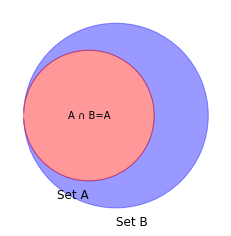
\includegraphics[width=8cm]{venn.png}
    
    \label*{Venn diagram}
\end{figure}

Option B) If $B \subset A$,
Then, 
\begin{align}
AB=B.
\end{align}
\begin{align}
\implies Pr(AB)=Pr(B)
\end{align}
But, from \eqref{1}, we have, 
\begin{align}
&Pr(AB)=Pr(A)\\
\implies &Pr(AB)=Pr(A)=Pr(B)
\end{align}
But,since A and B are two events, $A\neq B$. Hence, option (B) is incorrect.
\begin{align*}
\\
\end{align*}
Option C) If $B=\phi$
\begin{align}
\implies Pr(AB)=0
\end{align}From \eqref{1}, we know that,
\begin{align}
& Pr(AB)=Pr(A)\\
\implies & Pr(AB)=Pr(A)=0
\end{align}
But,from the given data, we know that $Pr(A) \neq 0$.\\
Therefore,option C is incorrect.
\begin{align*}
\\
\end{align*}
Option D) If $A=\phi$,
\begin{align}
\implies Pr(A)=0
\end{align}
But,from the given data, we know that $Pr(A) \neq 0$.\\
Therefore,option D is incorrect.
\end{document}